
\subsection{Move IIIa}
Let $A^\pm = A = \Z_2\<{a,b,c, a_1, ..., a_l}$ where $a,b$ and $c$ are as shown in
figure \pref{fig:move_iiia} and $a_1,...,a_l$ denote the crossing outside a
neighbourhood of the bifurcation. Note that the grading of $a,b$ and $c$
are the same in both diagrams and thus $A^+$ and $A^-$ are isomorphic as graded
vector spaces. We claim that $m^+ = m^-$. 
To prove this we will, by continuity, construct a bijective map
$R_k: W^+_k(\Ym) \to W^+_k(\Yp)$
such that for each $f \in W^+_k(\Ym)$ and vertex $x_i^k$ of $\Pi_k$, 
\[ R(f)(x_i^k) = f(x_i^k) \in \Z_2\<{a,b,c, a_1, ..., a_l}. \]
It then follows immediately that $m^+ = m^-$.

\begin{figure}
\centering
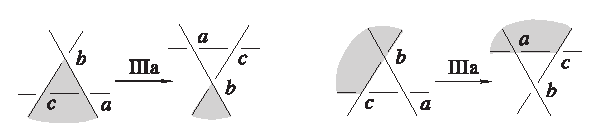
\includegraphics[width=.6\textwidth]{figs/move_iiia.pdf}
\caption{}
\label{fig:move_iiia}
\end{figure}

Let $f^\pm \in W^+_3(\Ypm)$ be the immersions whose image is
the small triangles with vertices $a,b,c$ and let $R(f_-)=f_+$. Then by Corollary
\pref{prop:height_sum}, 

\begin{equation}
\label{eq:habc}
H(a) > H(b) + H(c), 
\end{equation}

\begin{lemma}
\label{prop:habc}
Let $f\in W_k^+(\Ypm)\setminus\{f_\pm\}$, then neither of the
segments $[a,b], [b,c], [a,c]$ is the image of an edge of $\Pi_k$ under the
immersion $f$.
\end{lemma}

\begin{proof}
If $[a,b]$ (resp. $[a,c]$) is the image of an edge of $\Pi_k$, the vertex sent
$b$ (resp.  $c$) is positive and that sent to $a$ negative. Then
Corollary \ref{prop:height_sum} would imply $H(b) > H(a)$ (resp. $H(a) > H(c)$),
which would contradict \pref{eq:habc}. If $[b,c]$ is the image of an edge, both
$b$ and $c$ would be positive and thus $f$ would not be admissible.
\end{proof}

Assume $f \in W_k^+(\Ym)\setminus\{f_-\}$ such that one of the
vertices is mapped to $a,b$ or $c$. Then, by lemma \ref{prop:habc}, $f$ can be
deformed, continuously in $t$, to an immersion $R(f) \in W_k^+(\Yp)$
as shown in figure \ref{fig:move_iiia}. 

By changing the direction of time, the very same construction defines a map 
$R': W_k^+(\Yp) \to W_k^+(\Ym)$ which is inverse to $R$.
